\documentclass[xcolor={usenames,dvipsnames}]{beamer}
%\documentclass[trans]{beamer}

% generic packages, macro definitions

%\usepackage{color}
\usepackage{geometry}
\usepackage{graphicx}
\usepackage{amsmath}
\usepackage{amsfonts}
\usepackage{amssymb}
\usepackage{setspace}
\usepackage{nameref}

% A package for simple formatting of code listings
\usepackage{listings} 
\lstset{numbers=left, numberstyle=\tiny, numbersep=5pt} 
\lstset{
  basicstyle=\ttfamily\small,
  keywordstyle=\color{red!70!black},
  commentstyle=\color{green!50!black},
  breaklines=true,  defaultdialect=[90]fortran,  defaultdialect=[LaTeX]TeX,
  morecomment=[l]{!\ }% Comment only with space after !
}

\usepackage{xparse}
\usepackage{tikz}
\usetikzlibrary{matrix,backgrounds}
\pgfdeclarelayer{myback}
\pgfsetlayers{myback,background,main}

\tikzset{mycolor/.style = {line width=1bp,color=#1}}%
\tikzset{myfillcolor/.style = {draw,fill=#1}}%





% Animate a sequence of images
\usepackage{animate}

% Show movies by click, but with external viewer
\usepackage{multimedia}


\newcommand{\slidefoot}[1]{
  \vfill
  \hrule
  \vspace{.02\textheight}

  {\small #1}
}

\newcommand{\highlight}[1]{%
  \colorbox{green!50}{$\displaystyle#1$}}
  


% Define the basic About Flow beamer style
% define your beamer style


\mode<presentation>
{

  \setbeamertemplate{footline}[frame number]

%  \usetheme{Singapore} % linear navigation along the top
%  \usetheme{Warsaw} % linear navigation along the top
%  \usetheme{Pittsburg} % linear navigation along the top
  \usetheme{CambridgeUS} % linear navigation along the top
%  \usetheme{Madrid} % linear navigation along the top
  
%  \usefonttheme{professionalfonts}
  \usefonttheme[onlysmall]{structurebold}
}



% Unified colour, but feel free to adap to the colour scheme
% used at your institution/company:
\definecolor{afloblue}{RGB}{0,55,205}
\usecolortheme[named=afloblue]{structure}

% Partner logo on the left, replace with your logo and
% adjust size with 'height', depth from line with 'raisebox'
\def\instlogo{%
% \raisebox{6pt}{
\includegraphics[height=6ex]{QM60BlackOnLight}}%
%   \raisebox{6pt}{
\includegraphics[height=12ex]{ccfd3}}%
   \raisebox{0 pt}{\hspace{1 cm}
\includegraphics[height=0.8 cm]{logo_PW}}%
}
% White on Black Aboutflow logo (designed by Mateusz Gugala):
\def\aflologo{%
  \raisebox{-6 pt}{
\includegraphics[height=10ex]{AF-LOGO-v10}}%
}

\def\deptlogo{%
   \raisebox{0 pt}{
\includegraphics[height=0.8 cm]{ccfd3.png}}%
}

%\newcommand{\nologo}{\setbeamertemplate{logo}{}} % command to set the logo to nothing

\setbeamertemplate{footline}[text line]{%
       \parbox{.95\linewidth}{\vspace{-2pt}\hspace{-10pt}{
           \instlogo\hspace{2 pt} \deptlogo\hspace{1.8 cm}\aflologo
         }}
	\parbox{\linewidth}{
	\textcolor{Gray}{\hspace{10pt}\vspace*{2pt} \insertframenumber/\inserttotalframenumber}}}
         
%\setbeamertemplate{footline}{New template \insertframenumber}
\setbeamertemplate{navigation symbols}{}

%\setbeamercovered{dynamic}
\setbeamercovered{transparent=6}



% Tell includegraphics where to find figures:
\graphicspath{
{./}
{figures/},
}


\begin{document}

% A plain titlepage
\title[]
  {Unsteady adjoint optimization}

\subtitle{with grid adaptation}

\author[Part 2]{%
\vspace{5 mm}
  Sheikh Razibul Islam\\
  \vspace{0 mm}
%  Jacek Szumbarski\\[.5\baselineskip]
  Institute of Aeronautics and Applied Mechanics\\
  Warsaw University of Technology\\ 
  \vspace{3 mm}
  {srislam}@meil.pw.edu.pl}
%  \institute{\small%
%%              f.duddeck@qmul.ac.uk\\
%              About Flow: Beamer Template\\
%              Version 5, 12 July 2014}
  

%\date{\small\copyright:\ \  Jens-Dominik M\"uller, 2014}
%\date{\today}
\date{August 18, 2014}


\frame{\titlepage}


\newcommand{\noinstlogo}{\setbeamertemplate{logo}{}} % command to set the logo to nothing
% Alternative xample for a  titlepage written over an image, white on black
%
% Change the style for the front page, put in a background image.
\setbeamertemplate{background canvas}{%
  %\includegraphics[width=\paperwidth]{title-tip_2-dark}}
%  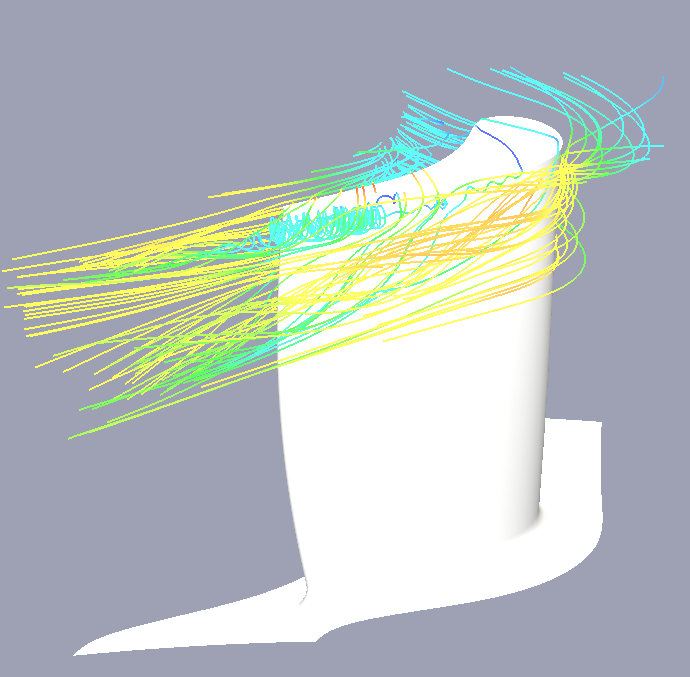
\includegraphics[width=\paperwidth]{title-tip_2-bright}}
    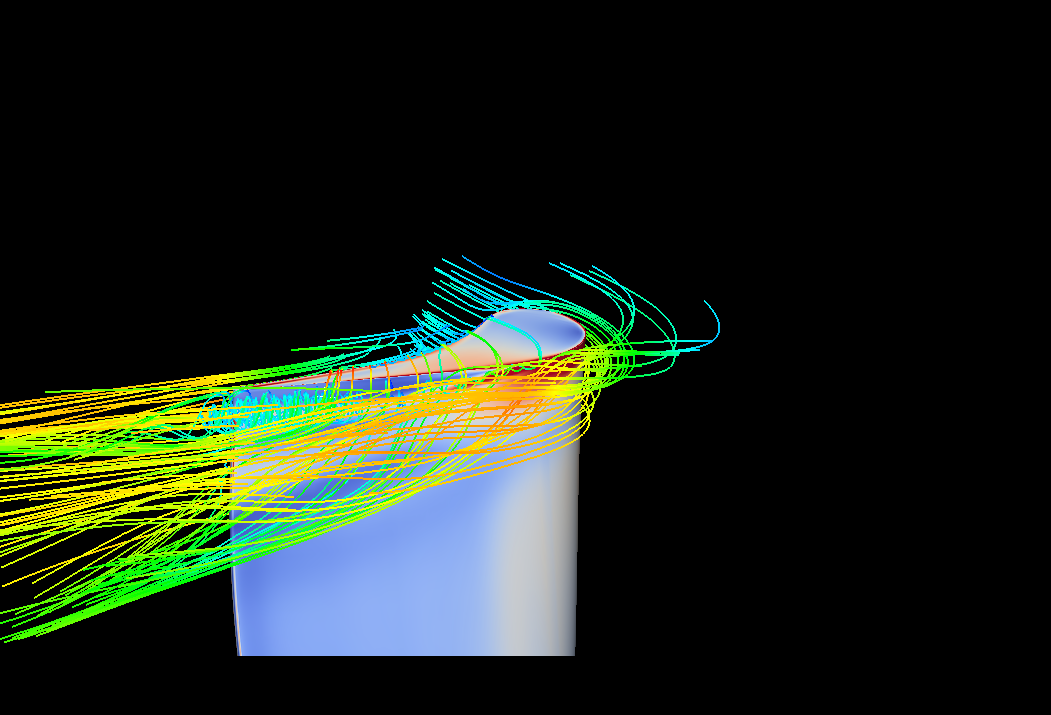
\includegraphics[width=14.2cm]{streamline7.png}}

\begin{frame}[plain]
  % titlepage; move things around to suit the image.
  % in this template a white font is used, thence the image
  % was darkened (gimp is your friend), and a white on dark logo
  % variant is used.
\vfill\vfill
\leftline{\color{white}\huge\bf Stabilisation of a discrete adjoint}
\center{\color{white}\huge\bf using implicit timestepping}
\vfill\vfill
\vfill\vfill\vfill\vfill

\rightline{\color{white}\bf Shenren Xu}
\rightline{\color{white}\bf Jens-Dominik M\"{u}ller}
\rightline{\color{white}\bf {Queen Mary, University of London}}
\vfill\vfill

\begin{columns}
  \begin{column}{.3\textwidth}
%    \includegraphics[width=\linewidth]{QM144BlueOnLight}
%   
\includegraphics[width=\linewidth]{ccfd3}
%	
\includegraphics[width=\linewidth]{WUT_L}
  \end{column}
  \begin{column}{.6\textwidth}
    \rightline{\color{white}\large \bf hydra implict meeting}
    \rightline{\color{white}\large \bf Derby, 10 April 2014}    
  \end{column}

\end{columns}


\end{frame}
\setbeamertemplate{background canvas}[default]


% Example for a  titlepage written over an image, dark on pale
%
% Change the style for the front page, put in a background image.
\setbeamertemplate{background canvas}{%
%  \includegraphics[width=\paperwidth]{title-tip_2-dark}}
  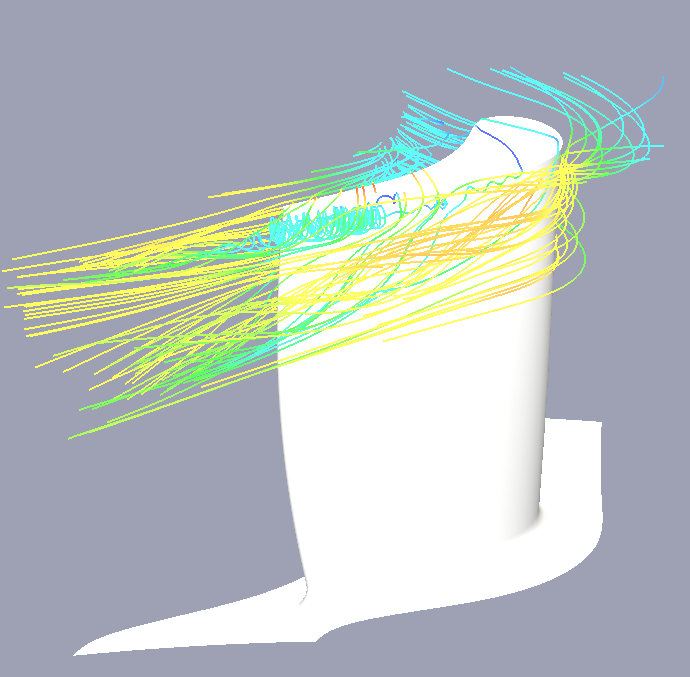
\includegraphics[width=\paperwidth]{title-tip_2-bright}}
%    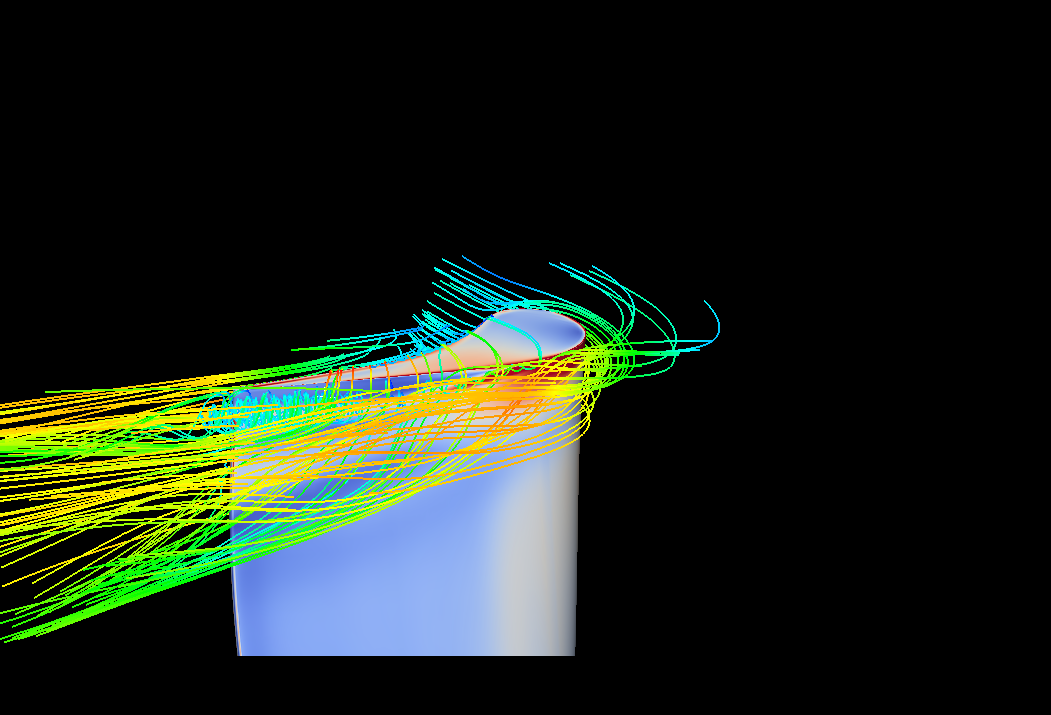
\includegraphics[width=14.2cm]{streamline7.png}}

\begin{frame}[plain]
  % titlepage; move things around to suit the image.
\vfill\vfill
\leftline{\color{black}\huge\bf Stabilisation of a discrete adjoint}
\center{\color{black}\huge\bf using implicit timestepping}
\vfill\vfill
\vfill\vfill\vfill\vfill

\rightline{\color{black}\bf Shenren Xu}
\rightline{\color{black}\bf Jens-Dominik M\"{u}ller}
\rightline{\color{black}\bf {Queen Mary, University of London}}
\vfill\vfill

\begin{columns}
  \begin{column}{.4\textwidth}
%    \includegraphics[width=\linewidth]{QM144BlueOnLight}
%   \includegraphics[width=\linewidth]{QM144WhiteOnDark}
%    
\includegraphics[width=\linewidth]{ccfd3}
    
\includegraphics[scale=0.05]{logo_PW}

  \end{column}
  \begin{column}{.6\textwidth}
    \rightline{\color{black}\large \bf hydra implict meeting}
    \rightline{\color{black}\large \bf Derby, 10 April 2014}    
  \end{column}

\end{columns}


\end{frame}
\setbeamertemplate{background canvas}[default]


% Example for a titlepage with a wrapped image.
%
% \title[Adjoint-based design optimisation] {Adjoint-based design
%   optimisation for steady and unsteady flows}
% \author[J.-D. M\"{u}ller]%
% {J.-D. M\"{u}ller \\
%   {\small Queen Mary, University of London}\\[10pt]
%   collaborators:\\
%   D.~Jones, S.~Xu, F.~Christakpoulos, W.~Jahn, M.~Oriani%, {\small QMUL}%
% %\\S.~Bayyuk, V.~Brown, {\small ESI} 
% }
% 
% \date{Imperial College, London,\\ 28 June 2013}




% Handcrafted title-page.
\setbeamertemplate{background canvas}{%
%  \begin{center}
%    \includegraphics[width=\textwidth]{flowfield}\\
%    
\includegraphics[width=\textwidth]{streamline2}
%  \end{center}
%  \includegraphics[height=\paperheight]{passat-front-right-crop}
}%
\begin{frame}[plain]
  %\titlepage
%\vfill
\leftline{\color{blue}\huge\bf Design optimisation}
\leftline{\color{blue}\huge\bf  for steady and unsteady flows}
\leftline{\color{blue}\huge\bf using adjoint methods}
\vfill\vfill
  \begin{center}
%    \includegraphics[width=\textwidth]{flowfield}\\
    
\includegraphics[width=\textwidth]{streamline2}
  \end{center}
\vfill\vfill

\leftline{\color{blue}\large\bf  Dr.~Jens-Dominik M\"{u}ller}
\leftline{\color{blue}\bf collaborators:}
\leftline{\color{blue}\bf 
          D.~Jones, F.~Christakpoulos, W.~Jahn, S.~Xu, M.~Oriani}
\leftline{\color{blue}\bf   {Queen Mary, University of London}}
\vfill

\begin{minipage}{\linewidth}
  \noindent
  \begin{minipage}[t]{.6\linewidth}
    \leftline{\color{blue} Fudan University, Shanghai, China}
    \leftline{\color{blue} 17 April 2013}
  \end{minipage} \hfil
  % \hspace{3 cm}
  \begin{flushright}
  
  \begin{minipage}{.3\linewidth}
%   \hspace{8cm}
   	  
\includegraphics[width=.3\linewidth]{logo_PW}
  \end{minipage}
  \end{flushright}
\end{minipage}
% \vfill
\end{frame}
\setbeamertemplate{background canvas}[default]





% Give an introduction, motivation, overview, before you
% get technical with a table of contents.
% % % % % % % % % % % % % % % % % % % % % % % % % % % % % % % % % % % % %

%\section*{Motivation} 
\newcommand{\ltx}[1]{{\tt \textbackslash#1}}
\begin{frame}{Personal Information}
\begin{block}{Background}
\begin{itemize}
\item Born in Khulna, Bangladesh
\item B.Sc. in Mechanical Engineering from Bangladesh University of Engineering \&Technology
%\item Worked for Metso Inc. as a Design Engineer
\item M.Sc. in Computational Mechanics from University of Duisburg-Essen,Germany
\end{itemize}
\end{block}
\begin{block}{Current Position}
\begin{itemize}
\item Joined WUT as ESR 14 on October, 2013
\item Supervised by Prof. Jacek Szumbarski
\end{itemize}
\end{block}
\end{frame}

\begin{frame}{Objectives}
\begin{block}{}
\begin{itemize}
\item Adjoint solver for unsteady Navier-Stokes (including check pointing)
\item Usage of adjoint calculation for shape optimization and optionally for optimal control
\item Optimize the performance with grid adaptation and optionally multi-gird
\end{itemize}
\end{block}
\end{frame}

\begin{frame}{Work Plan}

\begin{block}{Preliminaries}
\begin{itemize}\item Unsteady adjoint for a simple ODE with checkpointing
\item optimal control for simple ODE
\end{itemize}
\end{block}
\pause
\begin{block}{Prerequisites}
\begin{itemize}
\item Unsteady Euler/NS solver (Residual Distribution Scheme)
\end{itemize}
\end{block}
\pause
\begin{block}{Primary Task}
\begin{itemize}
\item Implementation of unsteady adjoint in the NS solver
\item Implementation of moving geometry
\item Gradient-based shape optimization
\end{itemize}
\end{block}

\end{frame}

\begin{frame}{Work Plan - continued}
\begin{block}{Testing and evaluation}
\begin{itemize}
\item Testing of the Euler/NS code on non-stationary cases
\item Testing of the obtained gradients against finite difference
\item Testing of a complete optimization
\end{itemize}
\end{block}
\begin{block}{Performance improvements}
\begin{itemize}
\item Hessian-of-solution based mesh refinement
\item Goal-oriented based mesh refinement
\end{itemize}
\end{block}
\end{frame}


%\begin{frame}{What this template is about}
%  \uncover<+->{This template provides a unified style, but
%    there is no requirement to adopt it. Use it, if you like it,
%    feel free to modify the colour scheme to match your
%    group style. 
%  \vfil
%  \uncover<+->{This is not an exhaustive explanation of latex
%    and beamer, there are lots of guides and help pages
%    around.}
%  \vfil
%  \uncover<+->{We just present typical elements we often use,
%    as well as suggesting some better practices. Hopefully this
%    is useful to save you time and help you make better presentations}
%   }
%  \vfil
%  \uncover<+->{You will need to replace the QM logo at the bottom left
%    with the logo of your group and/or institution. Look for the
%    macro \ltx{instlogo} in {\tt aflo\_beamer\_style.tex}.
%   }
%\end{frame}

\begin{frame}
\frametitle{Progress}
\begin{block}{Progress}
\begin{itemize}
\item Literature review
\item Training on adjoint-based mesh adaptation and optimization
\item Training on AD tools
\item Training on Open MPI
\item Development of Adjoint implementation on Euler solver is underway.
\end{itemize}
\end{block}
\end{frame}

\begin{frame}{Secondments}

\begin{block}{RWTH}
\begin{itemize}
\item Familiarization in parallelization of adjoint solvers
\item Review of AD tools for parallel application
\item Implementation of operator overloading based AD to develop Adjoint solver

\end{itemize}
\end{block}

\begin{block}{RR}
\begin{itemize}
\item Investigation of turbo-machinery problem using the developed adjoint solver 
\item Application of grid adaptation tool chain available in WUT for turbo-machinery test cases
\end{itemize}
\end{block}
\end{frame}

\begin{frame}{Duality Formulation For Adjoint Design}
\begin{block}{Primal:}
\begin{equation}
Q^{n+1}=F(Q^n)
\end{equation}
\end{block}
\begin{block}{Tangent Linear:}
\begin{equation}
\frac{\partial Q^{n+1}}{\partial \alpha} = \frac{\partial F}{\partial Q}\frac{\partial Q}{\partial \alpha} +\frac{\partial I}{\partial \alpha}
\end{equation}
\end{block}

\begin{block}{Adjoint Equation:}
\begin{equation}
v^n = \highlight{\left(\frac{\partial F}{\partial Q}\right)^{T}}v^{n+1} +\frac{\partial I}{\partial Q}
\end{equation}
\end{block}


\end{frame}

\begin{frame}{Advantage of Finite Difference to Develop Jacobian}
\tiny
%\begin{equation}
%\begin{bmatrix}
%a_{11}  & a_{12}  & 0   & \cdots & 0 \\
%a_{21}  & a_{22}  & a_{23}  & \ddots  & \vdots \\
%0 & a_{32}  & a_{33}   & \ddots  & \vdots \\
%%\vdots & \ddots & \ddots & \ddots & \ddots & \ddots &  & \vdots \\
%\vdots &  & \ddots  & \ddots& \vdots\\
%%\vdots  &  & & \ddots & a_{76}  & a_{77}  &  a_{78}  & 0\\
%%\vdots  &  & & & \ddots & a_{87}  & a_{88}  &  a_{89}\\
%0   & \cdots & 0 & a_{98} & a_{99}  \\
%\end{bmatrix}
%\end{equation}

%\begin{equation}
%\begin{bmatrix}
%a_{11}  & a_{12}  & 0 & \cdots & \cdots & \cdots & \cdots & 0 \\
%a_{21}  & a_{22}  & a_{23}  & \ddots & && & \vdots \\
%0 & a_{32}  & a_{33} & a_{34}  & \ddots & &  & \vdots \\
%\vdots & \ddots & \ddots & \ddots & \ddots & \ddots &  & \vdots \\
%\vdots & & \ddots & \ddots & \ddots & \ddots & \ddots& \vdots\\
%\vdots  &  & & \ddots & a_{76}  & a_{77}  &  a_{78}  & 0\\
%\vdots  &  & & & \ddots & a_{87}  & a_{88}  &  a_{89}\\
%0 & \cdots &  \cdots & \cdots & \cdots & 0 & a_{98} & a_{99}  \\
%\end{bmatrix}
%\end{equation}

\begin{equation}
\begin{bmatrix}
a_{11}  & a_{12}  & 0  & \cdots & \cdots & \cdots & 0 \\
a_{21}  & a_{22}  & a_{23}  & \ddots & &&  \vdots \\
0 & a_{32}  & a_{33} & a_{34}  & \ddots &   & \vdots \\
\vdots & & \ddots & \ddots & \ddots & \ddots& \vdots\\
\vdots  &   &  & a_{76}  & a_{77}  &  a_{78}  & 0\\
\vdots  &   & & \ddots & a_{87}  & a_{88}  &  a_{89}\\
0 & \cdots &  \cdots & \cdots & 0 & a_{98} & a_{99}  \\
\end{bmatrix}
\end{equation}
\normalsize
\begin{itemize}
\item Developed Jacobian is a complete sparse matrix which can be calculated locally
\item It is conveniently scalable
\item Options to implement higher order FDM, if more accurate jacobian is required
\item Tested for stationary problems with sufficient accuracy
\end{itemize}
\end{frame}


%\begin{frame}{Introduction, Table of Contents, Roadmap}
%  \uncover<+->{beamer provides a nice Table of Content
%    feature if you use the \ltx{section} command.}
%
%  \uncover<+->{There is little point in starting
%   your talk with a boring ToC, the audience will not know
%   what these headings mean. Much better to first give an 
%   overview/motivation, then give them a 'map' how you will be explaining
%   your work.}
%
%  \uncover<+->{All sections will appear in section listings on the
%    borders of the style (here at the very top). Since these listings
%    are to help orientate the audience, I don't think this is useful
%    before you've shown the ToC, hence it is commented out in the
%    source of this introductory part.}
%
%  \uncover<+->{Note, you could suppress the appearance of a section title
%   in the ToC if you use the \ltx{section*} command,
%   but it would still appear at the top of each frame.}
%\end{frame}

%\begin{frame}{What application are we aiming for?}
%  Example of itemisation coming up as a block using
%  the {\tt \textbackslash uncover} command:
%  \uncover<2->{
%  \begin{itemize}
%  \item All items
%  \item are shown
%  \item at once,
%  \end{itemize}
%  }
%
%  \uncover<3->{
%    Or items popping up one after the other:
%    \begin{itemize}
%    \item<4-> Note that when you look at the source of this frame, 
%    \item<6-> we explicitly number how things
%    \item<5-> come up.
%    \end{itemize}
%
%    \slidefoot{It is not very useful to give detailed lists of references
%      at the end, the audience can't flip back and forth in your
%      presentation. Better to provide a shortened reference at the relevant 
%      page:\\
%      T.~Tantau et al., ``The BEAMER class'', Dec 2013, tug.ctan.org }
%  }
%\end{frame}

%\begin{frame}{What is the problem that we address?}
%  \uncover<+->{While here}
%  \begin{itemize}
%  \item<+->we simply
%  \item <+-> increment.
%  \end{itemize}
%
%  \uncover<+->{But beware:}
%  \begin{itemize}
%  \item<+-> Avoid
%  \item<+-> uncovering 
%  \item<+-> too little
%  \item<+-> information
%  \item<+-> in too many
%  \item<+-> small 
%  \item<+-> steps
%  \end{itemize}
%\end{frame}

%\begin{frame}{Ready for the roadmap?}
%  Now that we set our work in context, we can show the Table 
%  of Contents.
%\end{frame}



%% Table of Contents, overview
%\begin{frame}
%\frametitle{Contents}
%\tableofcontents%[allsections,hidesubsections]
%\end{frame}

% This shows the ToC before each new section.
\AtBeginSection[]
{
\begin{frame}{Contents}
%   \frametitle{\insertsectionhead}
  \tableofcontents[currentsection,hideothersubsections]
\end{frame}
}


% Main body
%
% Section headings appear in the Table of contents
\section[Basic structuring]{Basic structuring: columns, relative sizes}
\begin{frame}{Structuring} 
  In the motivation section we have already seen how to
  use 
  \begin{itemize}
  \item paragraphs
  \item itemi[z]ation and
  \item uncover
  \end{itemize}
  to structure our frames [slides].

  \vfill
  \uncover<2->{There are a few other useful elements}
\end{frame}

\begin{frame}{Columns}
\parbox{\textwidth}{
  A nice and easy option to present information in columns with
  minimal work (certainly easier than using \ltx{minipage}) is
  to use columns:}

  \vfill

  \begin{columns}
    \begin{column}{.51\textwidth}
      \uncover<2->{Some text can go here and fill this
        column.

        Text will be formatted same as a full page.
        }      
    \end{column}
    \begin{column}{.4\textwidth}
      \uncover<3->{And some text can go here and fill this
        column.}
      \uncover<4->{
        Easy. 
        }
    \end{column}
  \end{columns}

\vfill
\uncover<5->{
I have used the \ltx{textwidth} variable to control the width of the columns.
You need to leave a bit of space between each columns, 0.09\ltx{textwidth} works
fine, so the width of my two columns sums to 0.91\ltx{textwidth}

\vfill
Note also the use of \ltx{vfill} to provide vertical rubber space
and help Latex to space the blocks out vertically on the frame.
}
\end{frame}


\section[Figures]{How to align and uncover figures}

\begin{frame}{How to (and how not to) include figures}
  Don't use the {\tt figure} environment in slides. {\tt figure}
  creates a ``floating body'' that Latex can place where best suited, 
  including the number and caption. Not what you want here. Use
  a straight \ltx{includegraphics}, and \ltx{centerline}
  to centre.

  \uncover<2-> {
  \ltx{includegraphics} can also be ``uncovered'', but if you
  want to reserve the space for the figure, i.e.~not have any
  preceding text move when the figure is shown, then you have
  to do a bit of extra work as in this example.
  }

  \invisible<1-2>{
    \centerline{
       \includegraphics<1-2>[width=.6\textwidth]{aflo-header}}         }
  \centerline{\includegraphics<3->[width=.6\textwidth]{aflo-header}}

  \uncover<4->{Remove the \ltx{invisible} image to see what happens
    without. You can see even with the phantom image, when you
    remove a bit of text, there is still a
    bit of a wobble, duckDuckGo is your friend to try
    other solutions.}
  
\end{frame}

\begin{frame}{Lining up figures in rows and columns}

You can either use the \ltx{tabular} environment and include
each figure in a box of the table, or simply line up with 
appropriate spacing. 

\vfill
Note that for Latex a graphic is just a
box, same as a letter, and will be lined up as a letter.

\vfill
%\begin{figure}
\hfil
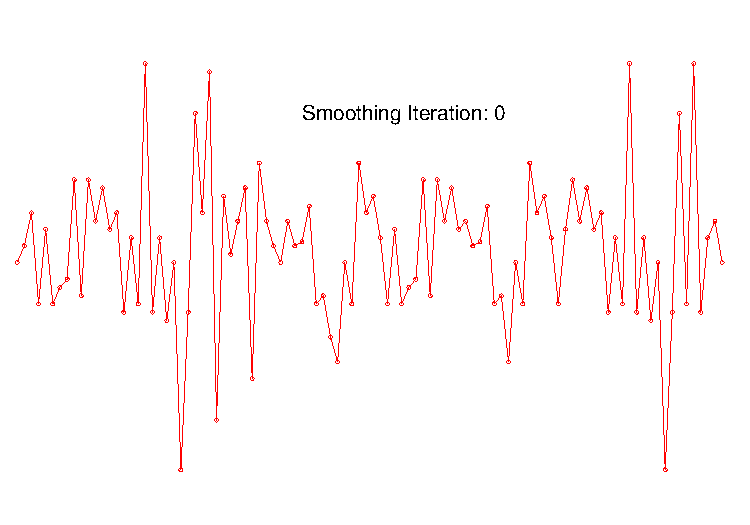
\includegraphics[width=.17\textwidth]{figures/animations/LaplacianSmoothing/smoothingEx-1}\hfil
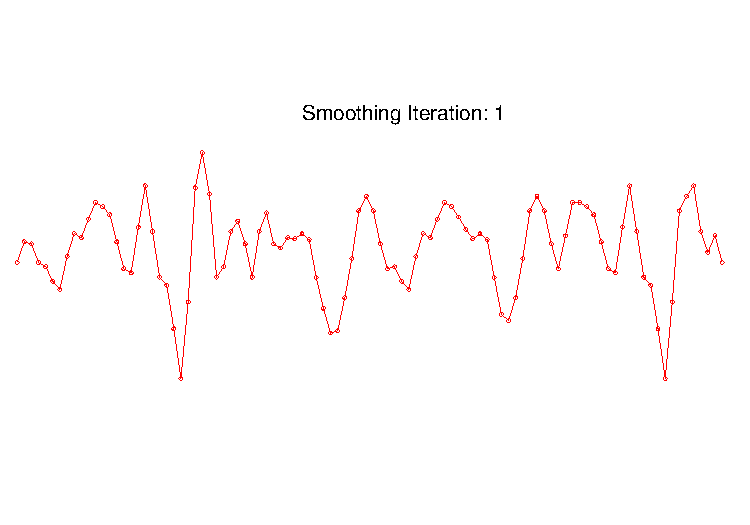
\includegraphics[width=.17\textwidth]{figures/animations/LaplacianSmoothing/smoothingEx-2}\hfil
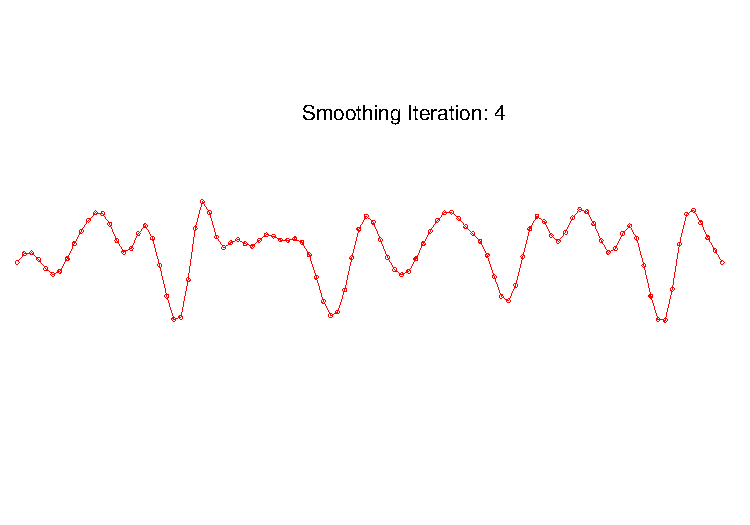
\includegraphics[width=.17\textwidth]{figures/animations/LaplacianSmoothing/smoothingEx-5}\hfil
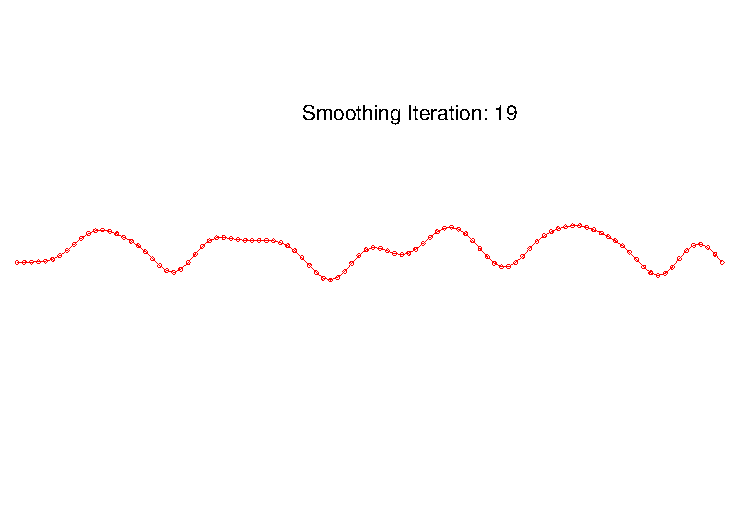
\includegraphics[width=.17\textwidth]{figures/animations/LaplacianSmoothing/smoothingEx-20}\hfil
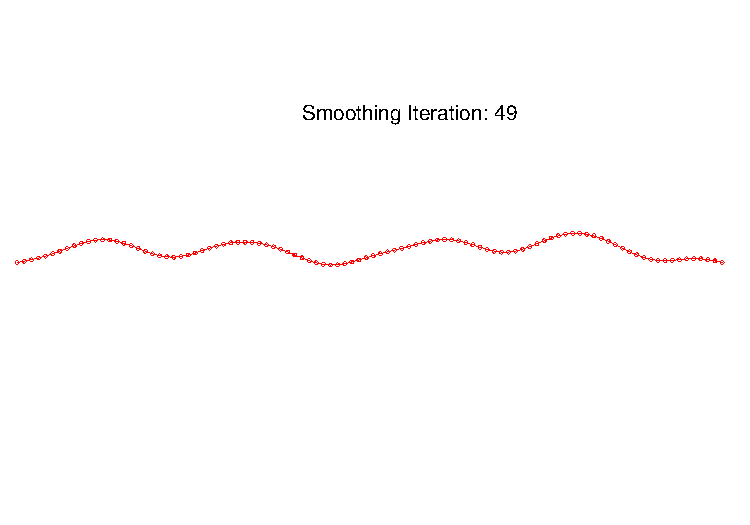
\includegraphics[width=.17\textwidth]{figures/animations/LaplacianSmoothing/smoothingEx-50}\hfil
%\end{figure}

%\smallskip

\hfil
\parbox{.17\textwidth}{\centerline{Iter 1  }}\hfil
\parbox{.17\textwidth}{\centerline{Iter 2  }}\hfil
\parbox{.17\textwidth}{\centerline{Iter 5  }}\hfil
\parbox{.17\textwidth}{\centerline{Iter 20 }}\hfil
\parbox{.17\textwidth}{\centerline{Iter 50 }}\hfil

\vfill
\uncover<2->{
Note the extensive use of relative measurements for figure scaling,
such as .17\ltx{textwidth}, rather than absolute measurements. This
also makes it easy to keep scalings when moving blocks of figures
between the paper and the talk.
}

\end{frame}


\begin{frame}{A neat and clean way to include graphics}
  \begin{itemize}
  \item Many tools (gnuplot, Inkscape, xfig) support output of Latex graphics
  \item Advantage: Full support of Latex typesetting, formulae etc.
  \item Text looks clean and has the right size. No more figures with unreadable text (Well, within a certain range of scaling).
  \item Image size can be changed without changing text size
  \item Gnuplot: use \texttt{set terminal epslatex size 10cm,7cm color; set output "example.eps"}
  \item Then run \texttt{epstopdf fd.eps} in terminal to create pdf image if you are using pdflatex
  \end{itemize}

\slidefoot{Contributed by JH}
\
\end{frame}


\begin{frame}{Example graphic produced with gnuplot}
  \begin{center}
    % GNUPLOT: LaTeX picture with Postscript
\begingroup
  \makeatletter
  \providecommand\color[2][]{%
    \GenericError{(gnuplot) \space\space\space\@spaces}{%
      Package color not loaded in conjunction with
      terminal option `colourtext'%
    }{See the gnuplot documentation for explanation.%
    }{Either use 'blacktext' in gnuplot or load the package
      color.sty in LaTeX.}%
    \renewcommand\color[2][]{}%
  }%
  \providecommand\includegraphics[2][]{%
    \GenericError{(gnuplot) \space\space\space\@spaces}{%
      Package graphicx or graphics not loaded%
    }{See the gnuplot documentation for explanation.%
    }{The gnuplot epslatex terminal needs graphicx.sty or graphics.sty.}%
    \renewcommand\includegraphics[2][]{}%
  }%
  \providecommand\rotatebox[2]{#2}%
  \@ifundefined{ifGPcolor}{%
    \newif\ifGPcolor
    \GPcolortrue
  }{}%
  \@ifundefined{ifGPblacktext}{%
    \newif\ifGPblacktext
    \GPblacktextfalse
  }{}%
  % define a \g@addto@macro without @ in the name:
  \let\gplgaddtomacro\g@addto@macro
  % define empty templates for all commands taking text:
  \gdef\gplbacktext{}%
  \gdef\gplfronttext{}%
  \makeatother
  \ifGPblacktext
    % no textcolor at all
    \def\colorrgb#1{}%
    \def\colorgray#1{}%
  \else
    % gray or color?
    \ifGPcolor
      \def\colorrgb#1{\color[rgb]{#1}}%
      \def\colorgray#1{\color[gray]{#1}}%
      \expandafter\def\csname LTw\endcsname{\color{white}}%
      \expandafter\def\csname LTb\endcsname{\color{black}}%
      \expandafter\def\csname LTa\endcsname{\color{black}}%
      \expandafter\def\csname LT0\endcsname{\color[rgb]{1,0,0}}%
      \expandafter\def\csname LT1\endcsname{\color[rgb]{0,1,0}}%
      \expandafter\def\csname LT2\endcsname{\color[rgb]{0,0,1}}%
      \expandafter\def\csname LT3\endcsname{\color[rgb]{1,0,1}}%
      \expandafter\def\csname LT4\endcsname{\color[rgb]{0,1,1}}%
      \expandafter\def\csname LT5\endcsname{\color[rgb]{1,1,0}}%
      \expandafter\def\csname LT6\endcsname{\color[rgb]{0,0,0}}%
      \expandafter\def\csname LT7\endcsname{\color[rgb]{1,0.3,0}}%
      \expandafter\def\csname LT8\endcsname{\color[rgb]{0.5,0.5,0.5}}%
    \else
      % gray
      \def\colorrgb#1{\color{black}}%
      \def\colorgray#1{\color[gray]{#1}}%
      \expandafter\def\csname LTw\endcsname{\color{white}}%
      \expandafter\def\csname LTb\endcsname{\color{black}}%
      \expandafter\def\csname LTa\endcsname{\color{black}}%
      \expandafter\def\csname LT0\endcsname{\color{black}}%
      \expandafter\def\csname LT1\endcsname{\color{black}}%
      \expandafter\def\csname LT2\endcsname{\color{black}}%
      \expandafter\def\csname LT3\endcsname{\color{black}}%
      \expandafter\def\csname LT4\endcsname{\color{black}}%
      \expandafter\def\csname LT5\endcsname{\color{black}}%
      \expandafter\def\csname LT6\endcsname{\color{black}}%
      \expandafter\def\csname LT7\endcsname{\color{black}}%
      \expandafter\def\csname LT8\endcsname{\color{black}}%
    \fi
  \fi
  \setlength{\unitlength}{0.0500bp}%
  \begin{picture}(5668.00,3968.00)%
    \gplgaddtomacro\gplbacktext{%
      \csname LTb\endcsname%
      \put(718,704){\makebox(0,0)[r]{\strut{}\scriptsize $10^{-10}$}}%
      \put(718,1030){\makebox(0,0)[r]{\strut{}\scriptsize $10^{-9}$}}%
      \put(718,1355){\makebox(0,0)[r]{\strut{}\scriptsize $10^{-8}$}}%
      \put(718,1681){\makebox(0,0)[r]{\strut{}\scriptsize $10^{-7}$}}%
      \put(718,2006){\makebox(0,0)[r]{\strut{}\scriptsize $10^{-6}$}}%
      \put(718,2332){\makebox(0,0)[r]{\strut{}\scriptsize $10^{-5}$}}%
      \put(718,2657){\makebox(0,0)[r]{\strut{}\scriptsize $10^{-4}$}}%
      \put(718,2983){\makebox(0,0)[r]{\strut{}\scriptsize $10^{-3}$}}%
      \put(718,3308){\makebox(0,0)[r]{\strut{}\scriptsize $10^{-2}$}}%
      \put(850,484){\makebox(0,0){\strut{}\scriptsize $10^{-12}$}}%
      \put(1726,484){\makebox(0,0){\strut{}\scriptsize $10^{-10}$}}%
      \put(2602,484){\makebox(0,0){\strut{}\scriptsize $10^{-8}$}}%
      \put(3478,484){\makebox(0,0){\strut{}\scriptsize $10^{-6}$}}%
      \put(4354,484){\makebox(0,0){\strut{}\scriptsize $10^{-4}$}}%
      \put(5230,484){\makebox(0,0){\strut{}\scriptsize $10^{-2}$}}%
      \put(80,2006){\rotatebox{90}{\makebox(0,0){\strut{}error}}}%
      \put(3259,154){\makebox(0,0){\strut{}Finite difference perturbation}}%
      \put(3259,3638){\makebox(0,0){\strut{}Validation of adjoint gradient wrt. finite differences}}%
    }%
    \gplgaddtomacro\gplfronttext{%
      \csname LTb\endcsname%
      \put(4945,3157){\makebox(0,0)[r]{\strut{}\scriptsize $\Vert\nabla_{FD}-\nabla_{adj}\Vert_2$}}%
    }%
    \gplbacktext
    \put(0,0){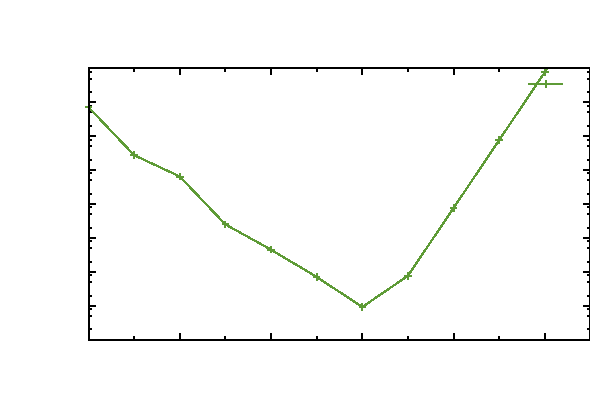
\includegraphics{fdvalidation}}%
    \gplfronttext
  \end{picture}%
\endgroup
    
  \end{center}
\end{frame}



\begin{frame}{And half the size}
  Some scaling can be done without re-running
  gnuplot by modifying the \ltx{setlength} statement in the 
  text part of the figure to an appropriate fraction, and then 
  adding a [scale=] optional argument to the \ltx{includegraphics}
  command. See the example in {\tt fdvalidation\_half.tex}.

  \begin{center}
    % GNUPLOT: LaTeX picture with Postscript
\begingroup
  \makeatletter
  \providecommand\color[2][]{%
    \GenericError{(gnuplot) \space\space\space\@spaces}{%
      Package color not loaded in conjunction with
      terminal option `colourtext'%
    }{See the gnuplot documentation for explanation.%
    }{Either use 'blacktext' in gnuplot or load the package
      color.sty in LaTeX.}%
    \renewcommand\color[2][]{}%
  }%
  \providecommand\includegraphics[2][]{%
    \GenericError{(gnuplot) \space\space\space\@spaces}{%
      Package graphicx or graphics not loaded%
    }{See the gnuplot documentation for explanation.%
    }{The gnuplot epslatex terminal needs graphicx.sty or graphics.sty.}%
    \renewcommand\includegraphics[2][]{}%
  }%
  \providecommand\rotatebox[2]{#2}%
  \@ifundefined{ifGPcolor}{%
    \newif\ifGPcolor
    \GPcolortrue
  }{}%
  \@ifundefined{ifGPblacktext}{%
    \newif\ifGPblacktext
    \GPblacktextfalse
  }{}%
  % define a \g@addto@macro without @ in the name:
  \let\gplgaddtomacro\g@addto@macro
  % define empty templates for all commands taking text:
  \gdef\gplbacktext{}%
  \gdef\gplfronttext{}%
  \makeatother
  \ifGPblacktext
    % no textcolor at all
    \def\colorrgb#1{}%
    \def\colorgray#1{}%
  \else
    % gray or color?
    \ifGPcolor
      \def\colorrgb#1{\color[rgb]{#1}}%
      \def\colorgray#1{\color[gray]{#1}}%
      \expandafter\def\csname LTw\endcsname{\color{white}}%
      \expandafter\def\csname LTb\endcsname{\color{black}}%
      \expandafter\def\csname LTa\endcsname{\color{black}}%
      \expandafter\def\csname LT0\endcsname{\color[rgb]{1,0,0}}%
      \expandafter\def\csname LT1\endcsname{\color[rgb]{0,1,0}}%
      \expandafter\def\csname LT2\endcsname{\color[rgb]{0,0,1}}%
      \expandafter\def\csname LT3\endcsname{\color[rgb]{1,0,1}}%
      \expandafter\def\csname LT4\endcsname{\color[rgb]{0,1,1}}%
      \expandafter\def\csname LT5\endcsname{\color[rgb]{1,1,0}}%
      \expandafter\def\csname LT6\endcsname{\color[rgb]{0,0,0}}%
      \expandafter\def\csname LT7\endcsname{\color[rgb]{1,0.3,0}}%
      \expandafter\def\csname LT8\endcsname{\color[rgb]{0.5,0.5,0.5}}%
    \else
      % gray
      \def\colorrgb#1{\color{black}}%
      \def\colorgray#1{\color[gray]{#1}}%
      \expandafter\def\csname LTw\endcsname{\color{white}}%
      \expandafter\def\csname LTb\endcsname{\color{black}}%
      \expandafter\def\csname LTa\endcsname{\color{black}}%
      \expandafter\def\csname LT0\endcsname{\color{black}}%
      \expandafter\def\csname LT1\endcsname{\color{black}}%
      \expandafter\def\csname LT2\endcsname{\color{black}}%
      \expandafter\def\csname LT3\endcsname{\color{black}}%
      \expandafter\def\csname LT4\endcsname{\color{black}}%
      \expandafter\def\csname LT5\endcsname{\color{black}}%
      \expandafter\def\csname LT6\endcsname{\color{black}}%
      \expandafter\def\csname LT7\endcsname{\color{black}}%
      \expandafter\def\csname LT8\endcsname{\color{black}}%
    \fi
  \fi
%  Original size:
%  \setlength{\unitlength}{0.0500bp}%
% Half the original size
  \setlength{\unitlength}{0.0250bp}%
  \begin{picture}(5668.00,3968.00)%
    \gplgaddtomacro\gplbacktext{%
      \csname LTb\endcsname%
      \put(718,704){\makebox(0,0)[r]{\strut{}\scriptsize $10^{-10}$}}%
      \put(718,1030){\makebox(0,0)[r]{\strut{}\scriptsize $10^{-9}$}}%
      \put(718,1355){\makebox(0,0)[r]{\strut{}\scriptsize $10^{-8}$}}%
      \put(718,1681){\makebox(0,0)[r]{\strut{}\scriptsize $10^{-7}$}}%
      \put(718,2006){\makebox(0,0)[r]{\strut{}\scriptsize $10^{-6}$}}%
      \put(718,2332){\makebox(0,0)[r]{\strut{}\scriptsize $10^{-5}$}}%
      \put(718,2657){\makebox(0,0)[r]{\strut{}\scriptsize $10^{-4}$}}%
      \put(718,2983){\makebox(0,0)[r]{\strut{}\scriptsize $10^{-3}$}}%
      \put(718,3308){\makebox(0,0)[r]{\strut{}\scriptsize $10^{-2}$}}%
      \put(850,484){\makebox(0,0){\strut{}\scriptsize $10^{-12}$}}%
      \put(1726,484){\makebox(0,0){\strut{}\scriptsize $10^{-10}$}}%
      \put(2602,484){\makebox(0,0){\strut{}\scriptsize $10^{-8}$}}%
      \put(3478,484){\makebox(0,0){\strut{}\scriptsize $10^{-6}$}}%
      \put(4354,484){\makebox(0,0){\strut{}\scriptsize $10^{-4}$}}%
      \put(5230,484){\makebox(0,0){\strut{}\scriptsize $10^{-2}$}}%
      \put(80,2006){\rotatebox{90}{\makebox(0,0){\strut{}error}}}%
      \put(3259,154){\makebox(0,0){\strut{}Finite difference perturbation}}%
      \put(3259,3638){\makebox(0,0){\strut{}Validation of adjoint gradient wrt. finite differences}}%
    }%
    \gplgaddtomacro\gplfronttext{%
      \csname LTb\endcsname%
      \put(4945,3157){\makebox(0,0)[r]{\strut{}\scriptsize $\Vert\nabla_{FD}-\nabla_{adj}\Vert_2$}}%
    }%
    \gplbacktext
%   Original include, unscaled.
%    \put(0,0){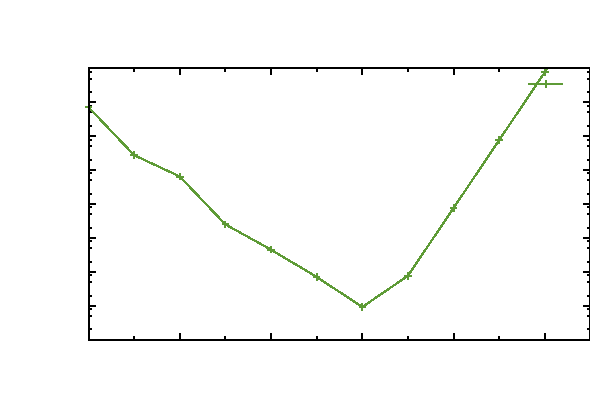
\includegraphics{fdvalidation}}%
%   Scaled-down include
    \put(0,0){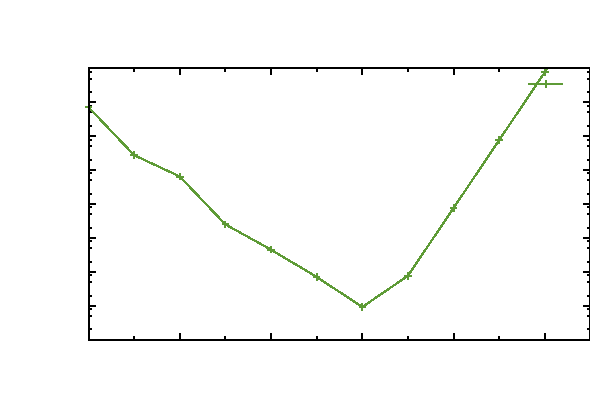
\includegraphics[scale=.5]{fdvalidation}}%
    \gplfronttext
  \end{picture}%
\endgroup
    
  \end{center}

  \uncover<2->{You can see that there are limits to scaling. But
   $\pm20\%$ is often ok.}
\end{frame}



\begin{frame}{Overlays}
 
  If you want to show different parts using the same space,
  then you can 'reserve' that space with \ltx{overlayarea}:

  \vfill

  \begin{overlayarea}{\textwidth}{.5\textheight}
    \only<1>{\centerline{% GNUPLOT: LaTeX picture with Postscript
\begingroup
  \makeatletter
  \providecommand\color[2][]{%
    \GenericError{(gnuplot) \space\space\space\@spaces}{%
      Package color not loaded in conjunction with
      terminal option `colourtext'%
    }{See the gnuplot documentation for explanation.%
    }{Either use 'blacktext' in gnuplot or load the package
      color.sty in LaTeX.}%
    \renewcommand\color[2][]{}%
  }%
  \providecommand\includegraphics[2][]{%
    \GenericError{(gnuplot) \space\space\space\@spaces}{%
      Package graphicx or graphics not loaded%
    }{See the gnuplot documentation for explanation.%
    }{The gnuplot epslatex terminal needs graphicx.sty or graphics.sty.}%
    \renewcommand\includegraphics[2][]{}%
  }%
  \providecommand\rotatebox[2]{#2}%
  \@ifundefined{ifGPcolor}{%
    \newif\ifGPcolor
    \GPcolortrue
  }{}%
  \@ifundefined{ifGPblacktext}{%
    \newif\ifGPblacktext
    \GPblacktextfalse
  }{}%
  % define a \g@addto@macro without @ in the name:
  \let\gplgaddtomacro\g@addto@macro
  % define empty templates for all commands taking text:
  \gdef\gplbacktext{}%
  \gdef\gplfronttext{}%
  \makeatother
  \ifGPblacktext
    % no textcolor at all
    \def\colorrgb#1{}%
    \def\colorgray#1{}%
  \else
    % gray or color?
    \ifGPcolor
      \def\colorrgb#1{\color[rgb]{#1}}%
      \def\colorgray#1{\color[gray]{#1}}%
      \expandafter\def\csname LTw\endcsname{\color{white}}%
      \expandafter\def\csname LTb\endcsname{\color{black}}%
      \expandafter\def\csname LTa\endcsname{\color{black}}%
      \expandafter\def\csname LT0\endcsname{\color[rgb]{1,0,0}}%
      \expandafter\def\csname LT1\endcsname{\color[rgb]{0,1,0}}%
      \expandafter\def\csname LT2\endcsname{\color[rgb]{0,0,1}}%
      \expandafter\def\csname LT3\endcsname{\color[rgb]{1,0,1}}%
      \expandafter\def\csname LT4\endcsname{\color[rgb]{0,1,1}}%
      \expandafter\def\csname LT5\endcsname{\color[rgb]{1,1,0}}%
      \expandafter\def\csname LT6\endcsname{\color[rgb]{0,0,0}}%
      \expandafter\def\csname LT7\endcsname{\color[rgb]{1,0.3,0}}%
      \expandafter\def\csname LT8\endcsname{\color[rgb]{0.5,0.5,0.5}}%
    \else
      % gray
      \def\colorrgb#1{\color{black}}%
      \def\colorgray#1{\color[gray]{#1}}%
      \expandafter\def\csname LTw\endcsname{\color{white}}%
      \expandafter\def\csname LTb\endcsname{\color{black}}%
      \expandafter\def\csname LTa\endcsname{\color{black}}%
      \expandafter\def\csname LT0\endcsname{\color{black}}%
      \expandafter\def\csname LT1\endcsname{\color{black}}%
      \expandafter\def\csname LT2\endcsname{\color{black}}%
      \expandafter\def\csname LT3\endcsname{\color{black}}%
      \expandafter\def\csname LT4\endcsname{\color{black}}%
      \expandafter\def\csname LT5\endcsname{\color{black}}%
      \expandafter\def\csname LT6\endcsname{\color{black}}%
      \expandafter\def\csname LT7\endcsname{\color{black}}%
      \expandafter\def\csname LT8\endcsname{\color{black}}%
    \fi
  \fi
%  Original size:
%  \setlength{\unitlength}{0.0500bp}%
% Half the original size
  \setlength{\unitlength}{0.0250bp}%
  \begin{picture}(5668.00,3968.00)%
 %   \gplgaddtomacro\gplbacktext{%
 %     \csname LTb\endcsname%
 %     \put(718,704){\makebox(0,0)[r]{\strut{}\scriptsize $10^{-10}$}}%
 %     \put(718,1030){\makebox(0,0)[r]{\strut{}\scriptsize $10^{-9}$}}%
 %     \put(718,1355){\makebox(0,0)[r]{\strut{}\scriptsize $10^{-8}$}}%
 %     \put(718,1681){\makebox(0,0)[r]{\strut{}\scriptsize $10^{-7}$}}%
 %     \put(718,2006){\makebox(0,0)[r]{\strut{}\scriptsize $10^{-6}$}}%
 %     \put(718,2332){\makebox(0,0)[r]{\strut{}\scriptsize $10^{-5}$}}%
 %     \put(718,2657){\makebox(0,0)[r]{\strut{}\scriptsize $10^{-4}$}}%
 %     \put(718,2983){\makebox(0,0)[r]{\strut{}\scriptsize $10^{-3}$}}%
 %     \put(718,3308){\makebox(0,0)[r]{\strut{}\scriptsize $10^{-2}$}}%
 %     \put(850,484){\makebox(0,0){\strut{}\scriptsize $10^{-12}$}}%
 %     \put(1726,484){\makebox(0,0){\strut{}\scriptsize $10^{-10}$}}%
 %     \put(2602,484){\makebox(0,0){\strut{}\scriptsize $10^{-8}$}}%
 %     \put(3478,484){\makebox(0,0){\strut{}\scriptsize $10^{-6}$}}%
 %     \put(4354,484){\makebox(0,0){\strut{}\scriptsize $10^{-4}$}}%
 %     \put(5230,484){\makebox(0,0){\strut{}\scriptsize $10^{-2}$}}%
 %     \put(80,2006){\rotatebox{90}{\makebox(0,0){\strut{}error}}}%
 %     \put(3259,154){\makebox(0,0){\strut{}Finite difference perturbation}}%
 %     \put(3259,3638){\makebox(0,0){\strut{}Validation of adjoint gradient wrt. finite differences}}%
 %   }%
 %   \gplgaddtomacro\gplfronttext{%
 %     \csname LTb\endcsname%
 %     \put(4945,3157){\makebox(0,0)[r]{\strut{}\scriptsize $\Vert\nabla_{FD}-\nabla_{adj}\Vert_2$}}%
 %   }%
    \gplbacktext
%   Original include, unscaled.
%    \put(0,0){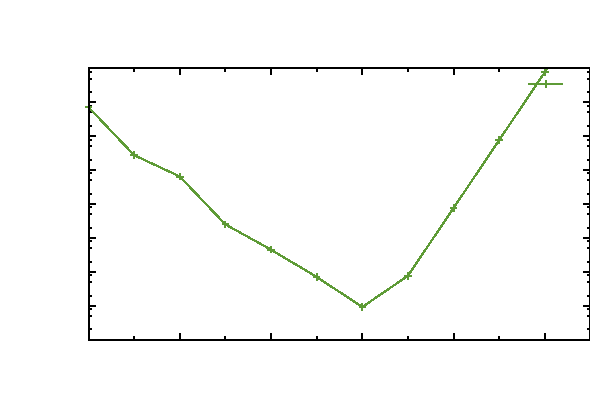
\includegraphics{fdvalidation}}%
%   Scaled-down include
    \put(0,0){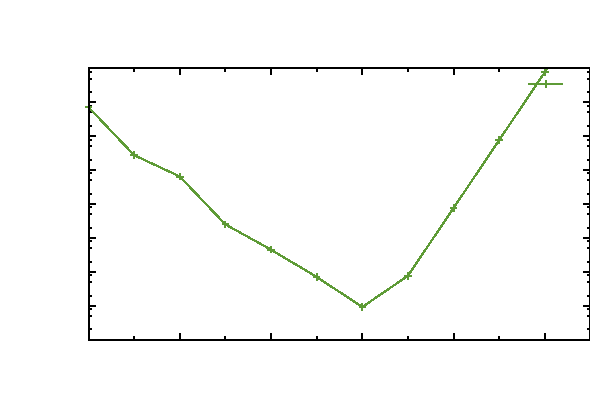
\includegraphics[scale=.5]{fdvalidation}}%
    \gplfronttext
  \end{picture}%
\endgroup
}}
    \only<2>{\centerline{% GNUPLOT: LaTeX picture with Postscript
\begingroup
  \makeatletter
  \providecommand\color[2][]{%
    \GenericError{(gnuplot) \space\space\space\@spaces}{%
      Package color not loaded in conjunction with
      terminal option `colourtext'%
    }{See the gnuplot documentation for explanation.%
    }{Either use 'blacktext' in gnuplot or load the package
      color.sty in LaTeX.}%
    \renewcommand\color[2][]{}%
  }%
  \providecommand\includegraphics[2][]{%
    \GenericError{(gnuplot) \space\space\space\@spaces}{%
      Package graphicx or graphics not loaded%
    }{See the gnuplot documentation for explanation.%
    }{The gnuplot epslatex terminal needs graphicx.sty or graphics.sty.}%
    \renewcommand\includegraphics[2][]{}%
  }%
  \providecommand\rotatebox[2]{#2}%
  \@ifundefined{ifGPcolor}{%
    \newif\ifGPcolor
    \GPcolortrue
  }{}%
  \@ifundefined{ifGPblacktext}{%
    \newif\ifGPblacktext
    \GPblacktextfalse
  }{}%
  % define a \g@addto@macro without @ in the name:
  \let\gplgaddtomacro\g@addto@macro
  % define empty templates for all commands taking text:
  \gdef\gplbacktext{}%
  \gdef\gplfronttext{}%
  \makeatother
  \ifGPblacktext
    % no textcolor at all
    \def\colorrgb#1{}%
    \def\colorgray#1{}%
  \else
    % gray or color?
    \ifGPcolor
      \def\colorrgb#1{\color[rgb]{#1}}%
      \def\colorgray#1{\color[gray]{#1}}%
      \expandafter\def\csname LTw\endcsname{\color{white}}%
      \expandafter\def\csname LTb\endcsname{\color{black}}%
      \expandafter\def\csname LTa\endcsname{\color{black}}%
      \expandafter\def\csname LT0\endcsname{\color[rgb]{1,0,0}}%
      \expandafter\def\csname LT1\endcsname{\color[rgb]{0,1,0}}%
      \expandafter\def\csname LT2\endcsname{\color[rgb]{0,0,1}}%
      \expandafter\def\csname LT3\endcsname{\color[rgb]{1,0,1}}%
      \expandafter\def\csname LT4\endcsname{\color[rgb]{0,1,1}}%
      \expandafter\def\csname LT5\endcsname{\color[rgb]{1,1,0}}%
      \expandafter\def\csname LT6\endcsname{\color[rgb]{0,0,0}}%
      \expandafter\def\csname LT7\endcsname{\color[rgb]{1,0.3,0}}%
      \expandafter\def\csname LT8\endcsname{\color[rgb]{0.5,0.5,0.5}}%
    \else
      % gray
      \def\colorrgb#1{\color{black}}%
      \def\colorgray#1{\color[gray]{#1}}%
      \expandafter\def\csname LTw\endcsname{\color{white}}%
      \expandafter\def\csname LTb\endcsname{\color{black}}%
      \expandafter\def\csname LTa\endcsname{\color{black}}%
      \expandafter\def\csname LT0\endcsname{\color{black}}%
      \expandafter\def\csname LT1\endcsname{\color{black}}%
      \expandafter\def\csname LT2\endcsname{\color{black}}%
      \expandafter\def\csname LT3\endcsname{\color{black}}%
      \expandafter\def\csname LT4\endcsname{\color{black}}%
      \expandafter\def\csname LT5\endcsname{\color{black}}%
      \expandafter\def\csname LT6\endcsname{\color{black}}%
      \expandafter\def\csname LT7\endcsname{\color{black}}%
      \expandafter\def\csname LT8\endcsname{\color{black}}%
    \fi
  \fi
%  Original size:
%  \setlength{\unitlength}{0.0500bp}%
% Half the original size
  \setlength{\unitlength}{0.0250bp}%
  \begin{picture}(5668.00,3968.00)%
    \gplgaddtomacro\gplbacktext{%
      \csname LTb\endcsname%
      \put(718,704){\makebox(0,0)[r]{\strut{}\scriptsize $10^{-10}$}}%
      \put(718,1030){\makebox(0,0)[r]{\strut{}\scriptsize $10^{-9}$}}%
      \put(718,1355){\makebox(0,0)[r]{\strut{}\scriptsize $10^{-8}$}}%
      \put(718,1681){\makebox(0,0)[r]{\strut{}\scriptsize $10^{-7}$}}%
      \put(718,2006){\makebox(0,0)[r]{\strut{}\scriptsize $10^{-6}$}}%
      \put(718,2332){\makebox(0,0)[r]{\strut{}\scriptsize $10^{-5}$}}%
      \put(718,2657){\makebox(0,0)[r]{\strut{}\scriptsize $10^{-4}$}}%
      \put(718,2983){\makebox(0,0)[r]{\strut{}\scriptsize $10^{-3}$}}%
      \put(718,3308){\makebox(0,0)[r]{\strut{}\scriptsize $10^{-2}$}}%
      \put(850,484){\makebox(0,0){\strut{}\scriptsize $10^{-12}$}}%
      \put(1726,484){\makebox(0,0){\strut{}\scriptsize $10^{-10}$}}%
      \put(2602,484){\makebox(0,0){\strut{}\scriptsize $10^{-8}$}}%
      \put(3478,484){\makebox(0,0){\strut{}\scriptsize $10^{-6}$}}%
      \put(4354,484){\makebox(0,0){\strut{}\scriptsize $10^{-4}$}}%
      \put(5230,484){\makebox(0,0){\strut{}\scriptsize $10^{-2}$}}%
      \put(80,2006){\rotatebox{90}{\makebox(0,0){\strut{}error}}}%
      \put(3259,154){\makebox(0,0){\strut{}Finite difference perturbation}}%
      \put(3259,3638){\makebox(0,0){\strut{}Validation of adjoint gradient wrt. finite differences}}%
    }%
    \gplgaddtomacro\gplfronttext{%
      \csname LTb\endcsname%
      \put(4945,3157){\makebox(0,0)[r]{\strut{}\scriptsize $\Vert\nabla_{FD}-\nabla_{adj}\Vert_2$}}%
    }%
    \gplbacktext
%   Original include, unscaled.
%    \put(0,0){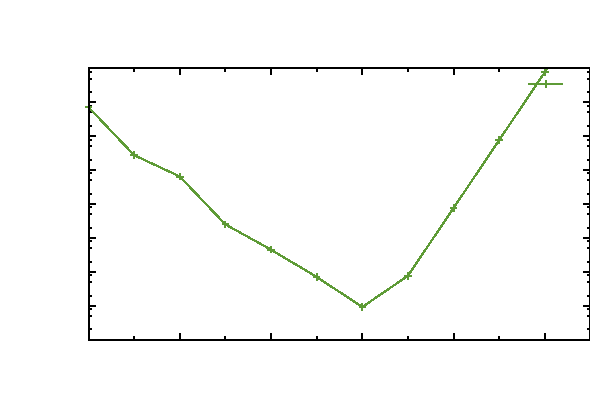
\includegraphics{fdvalidation}}%
%   Scaled-down include
    \put(0,0){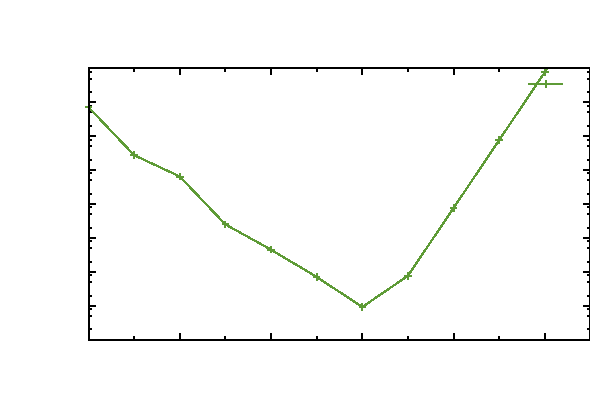
\includegraphics[scale=.5]{fdvalidation}}%
    \gplfronttext
  \end{picture}%
\endgroup
}}
    \only<3>{\centerline{% GNUPLOT: LaTeX picture with Postscript
\begingroup
  \makeatletter
  \providecommand\color[2][]{%
    \GenericError{(gnuplot) \space\space\space\@spaces}{%
      Package color not loaded in conjunction with
      terminal option `colourtext'%
    }{See the gnuplot documentation for explanation.%
    }{Either use 'blacktext' in gnuplot or load the package
      color.sty in LaTeX.}%
    \renewcommand\color[2][]{}%
  }%
  \providecommand\includegraphics[2][]{%
    \GenericError{(gnuplot) \space\space\space\@spaces}{%
      Package graphicx or graphics not loaded%
    }{See the gnuplot documentation for explanation.%
    }{The gnuplot epslatex terminal needs graphicx.sty or graphics.sty.}%
    \renewcommand\includegraphics[2][]{}%
  }%
  \providecommand\rotatebox[2]{#2}%
  \@ifundefined{ifGPcolor}{%
    \newif\ifGPcolor
    \GPcolortrue
  }{}%
  \@ifundefined{ifGPblacktext}{%
    \newif\ifGPblacktext
    \GPblacktextfalse
  }{}%
  % define a \g@addto@macro without @ in the name:
  \let\gplgaddtomacro\g@addto@macro
  % define empty templates for all commands taking text:
  \gdef\gplbacktext{}%
  \gdef\gplfronttext{}%
  \makeatother
  \ifGPblacktext
    % no textcolor at all
    \def\colorrgb#1{}%
    \def\colorgray#1{}%
  \else
    % gray or color?
    \ifGPcolor
      \def\colorrgb#1{\color[rgb]{#1}}%
      \def\colorgray#1{\color[gray]{#1}}%
      \expandafter\def\csname LTw\endcsname{\color{white}}%
      \expandafter\def\csname LTb\endcsname{\color{black}}%
      \expandafter\def\csname LTa\endcsname{\color{black}}%
      \expandafter\def\csname LT0\endcsname{\color[rgb]{1,0,0}}%
      \expandafter\def\csname LT1\endcsname{\color[rgb]{0,1,0}}%
      \expandafter\def\csname LT2\endcsname{\color[rgb]{0,0,1}}%
      \expandafter\def\csname LT3\endcsname{\color[rgb]{1,0,1}}%
      \expandafter\def\csname LT4\endcsname{\color[rgb]{0,1,1}}%
      \expandafter\def\csname LT5\endcsname{\color[rgb]{1,1,0}}%
      \expandafter\def\csname LT6\endcsname{\color[rgb]{0,0,0}}%
      \expandafter\def\csname LT7\endcsname{\color[rgb]{1,0.3,0}}%
      \expandafter\def\csname LT8\endcsname{\color[rgb]{0.5,0.5,0.5}}%
    \else
      % gray
      \def\colorrgb#1{\color{black}}%
      \def\colorgray#1{\color[gray]{#1}}%
      \expandafter\def\csname LTw\endcsname{\color{white}}%
      \expandafter\def\csname LTb\endcsname{\color{black}}%
      \expandafter\def\csname LTa\endcsname{\color{black}}%
      \expandafter\def\csname LT0\endcsname{\color{black}}%
      \expandafter\def\csname LT1\endcsname{\color{black}}%
      \expandafter\def\csname LT2\endcsname{\color{black}}%
      \expandafter\def\csname LT3\endcsname{\color{black}}%
      \expandafter\def\csname LT4\endcsname{\color{black}}%
      \expandafter\def\csname LT5\endcsname{\color{black}}%
      \expandafter\def\csname LT6\endcsname{\color{black}}%
      \expandafter\def\csname LT7\endcsname{\color{black}}%
      \expandafter\def\csname LT8\endcsname{\color{black}}%
    \fi
  \fi
%  Original size:
%  \setlength{\unitlength}{0.0500bp}%
% Half the original size
  \setlength{\unitlength}{0.0250bp}%
  \begin{picture}(5668.00,3968.00)%
    \gplgaddtomacro\gplbacktext{%
      \csname LTb\endcsname%
      \put(718,704){\makebox(0,0)[r]{\strut{}\scriptsize $10^{-10}$}}%
      \put(718,1030){\makebox(0,0)[r]{\strut{}\scriptsize $10^{-9}$}}%
      \put(718,1355){\makebox(0,0)[r]{\strut{}\scriptsize $10^{-8}$}}%
      \put(718,1681){\makebox(0,0)[r]{\strut{}\scriptsize $10^{-7}$}}%
      \put(718,2006){\makebox(0,0)[r]{\strut{}\scriptsize $10^{-6}$}}%
      \put(718,2332){\makebox(0,0)[r]{\strut{}\scriptsize $10^{-5}$}}%
      \put(718,2657){\makebox(0,0)[r]{\strut{}\scriptsize $10^{-4}$}}%
      \put(718,2983){\makebox(0,0)[r]{\strut{}\scriptsize $10^{-3}$}}%
      \put(718,3308){\makebox(0,0)[r]{\strut{}\scriptsize $10^{-2}$}}%
      \put(850,484){\makebox(0,0){\strut{}\scriptsize $10^{-12}$}}%
      \put(1726,484){\makebox(0,0){\strut{}\scriptsize $10^{-10}$}}%
      \put(2602,484){\makebox(0,0){\strut{}\scriptsize $10^{-8}$}}%
      \put(3478,484){\makebox(0,0){\strut{}\scriptsize $10^{-6}$}}%
      \put(4354,484){\makebox(0,0){\strut{}\scriptsize $10^{-4}$}}%
      \put(5230,484){\makebox(0,0){\strut{}\scriptsize $10^{-2}$}}%
      \put(80,2006){\rotatebox{90}{\makebox(0,0){\strut{}error}}}%
      \put(3259,154){\makebox(0,0){\strut{}Finite difference perturbation}}%
      \put(3259,3638){\makebox(0,0){\strut{}Validation of adjoint gradient wrt. finite differences}}%
    }%
    \gplgaddtomacro\gplfronttext{%
      \csname LTb\endcsname%
      \put(4945,3157){\makebox(0,0)[r]{\strut{}\scriptsize $\Vert\nabla_{FD}-\nabla_{adj}\Vert_2$}}%
    }%
    \gplbacktext
%   Original include, unscaled.
%    \put(0,0){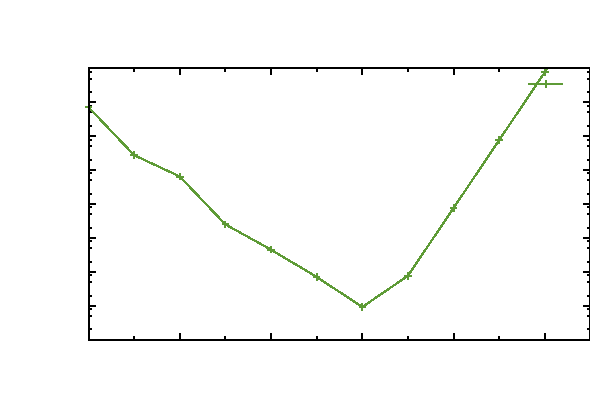
\includegraphics{fdvalidation}}%
%   Scaled-down include
%    \put(0,0){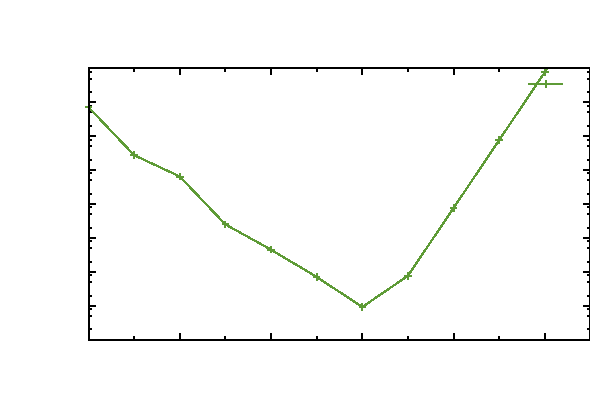
\includegraphics[scale=.5]{fdvalidation}}%
    \gplfronttext
  \end{picture}%
\endgroup
}}
  \end{overlayarea}

  \only<1>{\centerline{The graph only}}
  \only<2>{\centerline{Graph and Text}}
  \only<3>{\centerline{Text only}}
\end{frame}

\section[Animation]{``You gotta move it, move it!''}

\begin{frame}{Films}
  None of the Linux-based viewers allow you to embed a video, but
  you can launch your player with a click on the still image:

  \begin{columns}
    \begin{column}<+->{.4\textwidth}
      \movie[externalviewer]
      {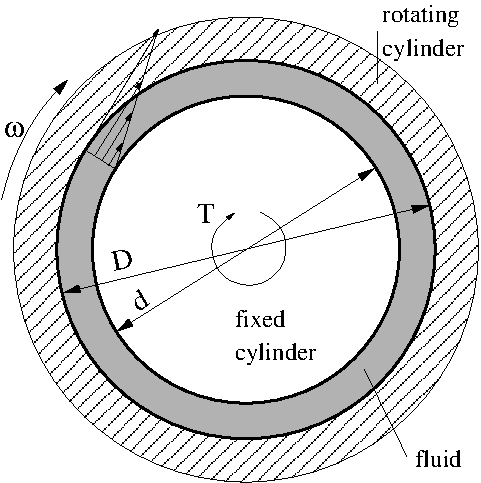
\includegraphics[width=\textwidth]{concentric_cylinder}}
      {figures/Glyzerin.mpg}
    \end{column}
    \begin{column}{.59\textwidth}
      \begin{itemize}
      \item You will need to install and add the {\tt multimedia}
      latex package.
        
      \item The player will not understand the \ltx{graphicspath}
      command, you need to explicitly give the path to the film.
    \item Mac and Windows pdf readers may be able to use embedded
      movies.
      \end{itemize}
    \end{column}
  \end{columns}

\end{frame}

\begin{frame}{Animations}
  For most of our shape optimisation work we only want to 
  show a few iterations, this is nicely done using {\tt animations}:

\centerline{
  % Find the manual at
  % http://ctan.math.utah.edu/ctan/tex-archive/macros/latex/contrib/animate/animate.pdf
  \animategraphics[loop,width=.5\textwidth]{6}
    {./figures/animations/LaplacianSmoothing/smoothingEx-}{1}{20}
  }
  You will need to include the {\tt animate} package.
  The Linux pdf reader evince won't understand this, but 
  Adobe's acroread does.  

  \slidefoot{Contributed by: Shenren, Mateusz}

\end{frame}

\section[Code]{A few ways of showing code}


\begin{frame}{Code example with columns and uncovering} 

  \begin{equation*}
    \mathbf{y} = 
  \left[
    \begin{array}{c}
      y_1 \\ y_2
    \end{array}
  \right]
  =
  \left[\begin{array}{l}
 \pi\cdot\cos(3x_1+2x_2+x_3)\cdot\pi\cdot\sin(3x_1+2x_2+x_3)\\   
 \pi\cdot\sin(3x_1+2x_2+x_3)\cdot x_1\\   
  \end{array}\right]
  \end{equation*}

  \vfill
  \begin{columns}
    \begin{column}<2->{.49\textwidth}
      {\small\tt
        u = 3*x(1)+2*x(2)+x(3) \\
        pi = 3.14 \\
        v = pi*cos(u) \\
        w = pi*sin(u) \\
        sum = v + u \\
        y(1) = v * w \\
        y(2) = w*x(1) \\
      }
    \end{column}
%
    \begin{column}{.49\textwidth}
      {\small\tt
        \uncover<6->{%
          gx(1) = 1\\ 
          gx(2) = gx(3) = 0\\
        }
        \uncover<5->{
          gu = 3*gx(1)+2*gx(2)+gx(3)\\}
        \uncover<4->{
          gv = -pi*sin(u)*gu\\
          gw = pi*cos(u)*gu\\
          gy(1) = gv*w + v*gw\\}
        \uncover<3->{        
          gy(2) = gw*x(1) + gx(1)*w\\}
      }
    \end{column}
  \end{columns}

%\source{Kaminski, Giering, 2002}, JDM added y(2)
\end{frame}


\begin{frame}{A simple example}
Full size font, indents controlled with \ltx{hspace} and variable
width.

\vfill
DO iter=1,n {\color{green}!Nonlinear iteration}\\
\hspace{0.6cm}DO istep=1,nstep{\color{green}!Runge-Kutta}\\
\hspace{1.2cm}IF(istep .EQ. 1) then\\
\hspace{1.8cm}		CALL {\color{blue}calc\_timestep}\\
\hspace{1.8cm}		CALL {\color{blue}calc\_jacob}\\
\hspace{1cm}\\
\hspace{1.2cm}    ENDIF	\\
\hspace{1.2cm}   CALL {\color{blue}calc\_res}\\
\hspace{1.2cm}   CALL {\color{blue}update}{\color{green}!SGS} \\
\hspace{0.6cm}ENDDO\\
\hspace{0.6cm}CALL {\color{blue}MG\_restriction/prolongation} {\color{green}!Multigrid}\\
\hspace{0.0cm}ENDDO

\end{frame}


\newcommand{\indt}{\hspace{.05\textwidth}}
\newcommand{\indth}{\hspace{.029\textwidth}}

\begin{frame}{A macro for the fixed space reduces typing}
  This example here uses a spacing macro \ltx{indt} to 
  create fixed indents (use it twice for double indentation). 
  
  And using a \ltx{small} font size.

  \vfill
  {\small 
    \uncover<2->{set $k=1$, $x_k = x_{start}$ \\} 
    \uncover<3->{\textbf{do}\\} 
    \uncover<4->{\indt compute $F(x_k)$, $\nabla F(x_k)$ \\} 
    \uncover<5->{\indt set $p_k = -\nabla F(x_k)$\\}
    \uncover<6->{\indt find $s$ to minimise $\varphi(s) = F(x_k\!+\!s p_k)$
          ! line search\\}
    \uncover<7->{\indt set $x_{k+1} = x_k + s p_k$\\}
    \uncover<3->{\textbf{while} $||\nabla F(x_k)|| \geq \varepsilon$ }
  }
\end{frame}


\begin{frame}[fragile]{A better example, using lslisting}
\begin{lstlisting}[gobble=2, language=Fortran]
  DO iter=1,n ! Nonlinear iteration
    DO istep=1,nstep ! Runge-Kutta
      IF(istep .EQ. 1) then
        CALL calc_timestep
        CALL calc_jacob
      ENDIF
      CALL calc_res
      CALL update !SGS
    ENDDO
    CALL MG_restriction/prolongation ! Multigrid
  ENDDO
\end{lstlisting}

\slidefoot{Proposed by: Jan}


\end{frame}

\begin{frame}[fragile]{How to input source code more easily}
Copy and paste this into your header:
\lstinputlisting[language=TeX, firstline=13, lastline=19]{talk.tex}
\end{frame}
\begin{frame}[fragile]{How to input source code more easily, cont'd}
Code can also be included from a file (ex.f90):
\lstinputlisting[language=Fortran, firstline=5, lastline=15]{ex.f90}
\end{frame}



\section{Summary}

\begin{frame}{Summary}

 
  It might be {\tt foo}

  \vfill
  But then Laurent says it is {\tt foo\_bar}

  \vfill
  \uncover<2->{
  We have now shown that it is simply \uncover<3->{\tt blah}}, 
  \uncover<4->{or actually {\tt diblah} and then {\tt obladibladah}}.
\end{frame}



% Keep this acknowledgements page as a reference to the EU.
%\section*{Acknowledgements}

\begin{frame}{Acknowledgements}
\
  This work has been conducted within the {\bf About Flow} project on
  \centerline{``Adjoint-based
  optimization of industrial and unsteady flows''.}
  \vfill
  \centerline {\tt http://aboutflow.sems.qmul.ac.uk}

  \vfill\vfill
  \begin{columns}
    \begin{column}{.55\textwidth}
    About Flow has received funding from the European Union's
    Seventh Framework Programme for research, technological development
    and demonstration under Grant Agreement No.~317006.
    \end{column}
    \begin{column}{.36\textwidth}
      
\includegraphics[width=\columnwidth]{EU}
    \end{column}
  \end{columns}
    
\vfill\vfill
\hfil

\includegraphics[width=0.49\textwidth]{Logo-Industry}
\hfil

\includegraphics[width=0.49\textwidth]{Logo-UNIs}
\hfil

\vspace{-.1\textheight}

\end{frame}


\end{document}
